\chapter{Обзор предметной области и постановка задачи}

\section{Динамическая и статическая трансляция}

\begin{Def}\label{binary_translation}
Бинарная трансляция - эмуляция одного набора инструкций через другой набор инструкций, т. е. трансляция последовательности инструкций исходного набора в эквивалентную последовательность инструкций целевого набора команд.
\end{Def}

В зависимости от необходимости исполнения исходной последовательности инструкций бинарную трансляцию разделяют на статическую и динамическую.

Статическая трансляция не подразумевает интерпретацию исходной последовательности, в то время как динамическая трансляция подразумевает интерпретацию исходной последовательности команд.

Технологии бинарной трансляции используются очень широко, например, виртуальные машины Java и .NET преобразуют байт-код в машинный код целевой платформы, что является частным случаем бинарной трансляции.

QEMU осуществляет бинарную трансляцию для эмуляции набора команд одного процессора на другом, что позволяет использовать его, например, вместо реального аппаратного обеспечения при разработке программных продуктов.

Популярный профилировщик Valgrind осуществляет бинарную трансляции в свое внутренне представление VEX IR~\footnote{http://www.valgrind.org/docs/manual/writing-tools.html}, в котором проще инструментировать код.

\subsection{Статическая трансляция}

В связи с необходимости сохранения семантики исходной последовательности команд, например, атомарность определенных инструкций, статическая трансляция является довольно сложной, кроме того, как я уже писал выше, имея только исполняемый файл в общем случае нельзя отличить бинарный код от данных программы без интерпретации бинарного кода, что ограничивает применение этого подхода.

Существуют различные реализации статических трансляторов, например, Ngen~\footnote{http://en.wikipedia.org/wiki/Native\_Image\_Generator} производит статическую трансляцию CIL в бинарный код целевой платформы, аналогичные средства есть для байт-кода Java~\footnote{http://en.wikipedia.org/wiki/GNU\_Compiler\_for\_Java}~\footnote{http://en.wikipedia.org/wiki/Excelsior\_JET}.

Следует отметить, что технологии статической трансляции могут применяться не только для преобразования последовательностей инструкций из разных наборов команд, но и для преобразования последовательности команд в рамках одного набора инструкций, например, с целью оптимизации~\footnote{http://www.cs.arizona.edu/projects/alto/}.

\subsection{Динамическая трансляция}\label{dynamic_translation}

По сравнению со статической динамическая трансляция имеет меньше ограничений, но за большую свободу часто приходится платить меньшей производительностью из-за накладных расходов на интерпретацию, которых нет при статической трансляции.

Однако не всегда производительность динамической трансляции ниже. Для ускорения может применяться техника Just In Time (JIT) компиляции, когда последовательности инструкций исходной платформы компилируются "на лету" в набор инструкций целевой платформы, что уменьшает накладные расходы. Кроме того при использовании JIT возможно использование оптимизаций недоступных при статической трансляции. Так JIT компилятору доступна, например, информация о наиболее горячих участках программы, что позволяет сгенерировать более быстрый, по сравнению со статически сгенерированным, бинарный код.

В качестве примеров динамических трансляторов можно привести виртуальные машины Java и .NET, а в качестве примера транслятора нативного кода QEMU и Valgrind.

В данной работе в качестве динамическо транслятора используется QEMU, так как он поддерживает множество аппаратных платформ (в том числе и arm), а кроме того имеет режим User Mode (для Linux и Free BSD), в котором он виртуализует не целую вычислительную систему, а только окружение одного процесса и осуществляет трансляцию системных вызовов исходной платформы (в рамках данной работы x86) в системные вызовы целевой (в рамках данной работы arm).

\subsection{QEMU}\label{qemu}

QEMU - динамический транслятор и эмулятор аппаратного обеспечения, автором которого является Фабрис Беллард~\footnote{http://en.wikipedia.org/wiki/Fabrice\_Bellard}. QEMU поддерживает эмуляцию большого количества архитектур, среди которых:

\begin{itemize}
    \item x86 и x86\_64
    \item arm
    \item sparc
    \item powerpc
    \item mips
    \item m86k
    \item и др.
\end{itemize}

QEMU может запускаться на следующих архитектурах:

\begin{itemize}
    \item x86 и x86\_64
    \item powerpc
    \item alpha
    \item sparc
    \item arm
    \item s390
    \item и др.
\end{itemize}

\paragraph{Блоки трансляции и кеш блоков трансляции.} Динамический транслятор QEMU использует честную трансляцию (straightforward), т. е. каждая инструкция разбивается на микрооперации, каждая из которых транслируется в фиксированный бинарный код. Такой подход обеспечивает высокую портируемость транслятора, относительную простоту, однако запрещает некоторые оптимизации кода.

Так как QEMU - динамический транслятор, код транслируется блоками. Блоки оканчиваются инструкциями, которые изменяют состояния процессора таким образом, что его нельзя определить без исполнения программы. Каждый такой блок называется блоком трансляции. Оттранслированные блоки сохраняются в кеше трансляции, который занимает 16 Mb~\cite{qemu}. Надо отметить, что с учетом локальности кода, блок выпадает из кеша довольно редко.

Состояние процессора, которое известно на этапе трансляции называется статическим состоянием, например, указатель инструкций является частью статического состояния, а условные переходы изменяют указатель инструкций и при этом без исполнения кода нельзя определить каким именно образом, поэтому инструкция перехода всегда заканчивает блок трансляции.

\paragraph{Алокация регистров.} QEMU использует очень примитивную фиксированную аллокацию регистров, т. е. каждый регистр целевого (гостевого или эмулируемого) процессора отображается на некоторый регистр хост процессора или регион памяти (чаще последнее). Такой метод является простым и легко переносимым, однако время доступа к памяти гораздо ниже времени доступа к регистрам, что приводит к значительной деградации производительности.

\paragraph{Связывание блоков трансляции.} После завершения исполнения оттранслированного блока, управление возвращается основному циклу QEMU, который зная состояние виртуального процессора проверяет, находится ли следующий блок в кеше трансляции или нет. Если блок находится в кеше трансляции, то управление передается ему, в противном случае необходимо оттранслировать блок.

С учетом локальности кода, довольно часто последовательности исполняемых блоков повторяются, в этом случае можно ускорить исполнение избежав передачи управления основному циклу QEMU, для этого необходимо в конец блока трансляции вставить проверку адреса следующего блока. Если адрес совпадает с ожиданиями, а это довольно часто так, то управление передается непосредственно по этому адресу, в противном случае, используется обычная передача управления основному циклу QEMU.

\section{Существующие реализации миграции}

Как отмечалось в пункте~\ref{migration_applications}, существует множество реализаций технологии миграции процессов, рассмотрим подробнее наиболее близкие к тематике данной работы.

\subsection{Linux-cr}
\label{linux_cr}

Проект по реализации технологии checkpoint/restore в ядре Linux~\footnote{https://ckpt.wiki.kernel.org/index.php/Main\_Page}. На данный момент проект не выглядит активным, последняя активность в ноябре 2010 года~\cite{linux_cr_lwn_report}. На момент последней активности код состоял из около 100 патчей в ядро Linux и содержал порядка 23 000 строк кода.

Основной проблемой проекта была попытка реализации проекта в пространстве ядра, так как он затрагивает большое количество подсистем, что усложняет поддержку и развитие проекта, а ошибки в системе миграции влияют на работу всей системы, делая ядро хрупким. Именно поэтому в своей работе я стараюсь минимизировать вмешательство в ядро Linux и получить как можно больше информации в пространстве пользователя.

Проект обладает достаточно большим списком поддерживаемых возможностей, кроме того поддерживает несколько архитектур: x86, x86\_64, PowerPC, s390 и arm.

Список реализованных возможностей:

\begin{itemize}

    \item поддержка многопоточных программ
    \item поддержка мьютексов
    \item поддержка сигналов
    \item файловые дескрипторы и директории для различных файловых систем
    \item файлы устройств (/dev/null, /dev/zero, /dev/random, /dev/urandom)
    \item поддержка epoll и event
    \item поддержка сокетов unix, ipv4 и ipv6 сокетов

\end{itemize}

но даже этот список не описывает все ресурсы, которые необходимо поддержать для полноценной миграции процессов.

\subsection{CRIU}

CRIU проект по реализации технологии checkpoint/restore преимущественно в пространстве пользователя Linux~\footnote{http://criu.org/Main\_Page}. Проект развивается при поддержке компании Paralles и находится в активной разработке.

Поддерживаемые возможности:

\begin{itemize}

    \item сохранение и восстановление TCP соединений
    \item сохранение и восстановление файловых дескрипторов
    \item поддержка многопоточных программ
    \item поддержка со стороны mainstream ядра

\end{itemize}

К сожалению, CRIU поддерживает только платформу x86\_64, что делает его неприменимым для кросс-архитектурной миграции процессов.

\subsection{DMTCP}

Проект по реализации технологии checkpoint/restart на уровне библиотек~\footnote{http://dmtcp.sourceforge.net/index.html}. Проект развивается, возможно, не очень активно, последняя версия 1.2.7 выпущена 13 марта 2013 года. Принцип работы заключается в запуске целевого процесса в специальном окружении, которое позволяет перехватывать некоторые вызовы и таким образом отслеживать состояние. DMTCP реализован в пространстве пользователя и поддерживает как многопоточные так и распределенные системы.

В связи с тем, что отслеживание состояния происходит во время работы процесса за счет перехвата библиотечных вызовов, существует некоторое падение производительности. Кроме того возможности этого проекта нужно оценивать уже не на уровне ресурсов ОС, а на уровне поддерживаемых библиотек и приложений.

На данный момент, DMTCP поддерживает следующие приложения и библиотеки:

\begin{itemize}

    \item MPI (в частности MPICH2)
    \item MATLAB
    \item Python
    \item Perl
    \item GNU screen
    \item X Window приложения без расширений (например, без OpenGL)
    \item и многие другие

\end{itemize}

Следует отметить, что такая реализация потенциально небезопасна~\footnote{http://criu.org/Comparison\_to\_other\_CR\_projects}. Например, DMTCP умеет перехватывать библиотечный вызов getpid, возвращая поддельный pid процесса, который может не соответствовать настоящему, но если, этот идентификатор используется для доступа, например, к файловой системе proc, тогда, без дополнительной трансляции имен файлов, процесс попытается обратиться к неправильному файлу - файлу другого процесса или несуществующему файлу, хотя в случае поддержки на уровне приложений, это, вероятно, не является проблемой.

\subsection{BLCR}

Проект по реализации checkpoint/restart лаборатории Berkeley~\footnote{https://ftg.lbl.gov/projects/CheckpointRestart/}. Проект направлен на гибридную (пространство пользователя/пространство ядра) реализацию checkpoint/restart не требующую изменения в коде приложения. Проект сосредоточен на параллельных и распределенных приложениях использующих MPI. Поддержка в ядре Linux не требует внесения специальных изменений в ядро и поставляется в виде набора модулей ядра.

Проект не выглядит активным, последняя версия 0.8.4 вышла 11 октября 2011 года, и начиная с 2008 года изменения содержат только исправления ошибок.

На момент последней активности проект имел стабильную поддержку архитектур x86 и x86\_64, а также экспериментальную поддержку PowerPC, PowerPC64 и arm, но кросс-архитектурная трансляции не поддерживается. Кроме того, как и DMTCP проект требует предварительно загрузки вспомогательных библиотек вместе с целевым процессом.

\subsection{Миграция виртуальных машин}

Кроме миграции отдельных процессов существует миграция целых виртуальных машин, эти технологии достаточно хорошо развиты и могут использоваться в практических целях. Например, гипервизор Xen позволяет осуществлять живую миграцию без остановок сервисов, т. е. без явных фаз создания образа и восстановления.~\footnote{http://en.wikipedia.org/wiki/Xen}.

Средства сохранения состояния виртуальной машины (snapshot) также есть у Virtual Box~\footnote{http://en.wikipedia.org/wiki/VirtualBox}, что, по факту, является другим названий для checkpoint/restart.

Несмотря на то, что технологии миграции в гипервизорах очень высоко развиты, они не способны выполнять кросс-архитектурную миграцию, и единственной достаточно функциональной виртуальной машиной с поддержкой различных архитектур.

\section{Цель работы}\label{aims}

Целью моей работы является реализация технологии кросс-архитектурной трансляции процессов ОС Linux с архитектуры x86 на arm на основе динамического транслятора QEMU. Для достижения указанной цели необходимо решить следующие задачи:

\paragraph{Анализ существующих решений.}

Необходимо рассмотреть существующие реализации технологии миграции процессов, а также принципы работы динамического транслятора QEMU.

\paragraph{Реализация технологии останова процесса и создания образа.}

Необходимо реализовать технологию создания образа процесса, сохраняющую минимально необходимый для восстановления набор ресурсов процесса - память и состояние регистров процессора. Основными принципами, которых нужно придерживаться при проектировании являются:

\begin{itemize}

    \item минимальное вмешательство в ядро Linux. Причиной этому является неудачный опыт проекта Linux-cr (см.~\ref{linux_cr}), в котором изменения затрагивали очень большое количество подсистема ядра, что сделало проект трудно поддерживаемым.

    \item необходимо наличие готового прототипа. Подход основанный на динамической трансляции создает дополнительные накладные расходы, возможность оценки этих расходов представляет интерес для выбора направлений дальнейшего развития, что делает важным получение рабочего прототипа для проведения тестов. Кроме того в рамках данной работы рассматривается возможность построения технологии кросс-архитектурной миграции, на данный момент цели построить полноценный набор средств для миграции любых процессов не стоит.

    \item архитектура расширяемая на новые платформы. В ходе работы рассматривается только миграция с архитектуры x86 на arm, так как у меня в наличии arm устройство, на котором можно тестировать результаты работы, однако технология кросс-архитектурной миграции не должна ограничиваться только двумя платформами.

\end{itemize}

\paragraph{Реализация восстановления процесса по образу.}

Необходимо реализовать восстановление процесса в динамическом трансляторе QEMU портированном на архитектуру arm.

\paragraph{Тестирование производительности.}

Динамическая трансляция, несомненно, создает дополнительные расходы, кроме того, процессоры архитектуры arm, как правило, менее производительны, чем процессоры x86, а численные оценки потерь производительности могут дать представление о границах применимости разрабатываемой технологии.

\section{Ресурсы процесса}

\begin{Def}\label{process}
Процесс - контейнер ресурсов операционной системы.
\end{Def}

Согласно определению~\ref{process}, миграция процесса - перенос ресурсов между вычислительными системами, вот далеко не полный перечень ресурсов, которые необходимо переносить:

\begin{itemize}

    \item память
    \item контекст процесса
    \item открытые файлы и директории (обычные и файлы устройств)
    \item сокеты
    \item мьютексы
    \item различные IPC примитивы

\end{itemize}

В рамках данной работы принято решение сосредоточится на двух основных ресурсах процесса: память и контекст (состояние процессора). Эти два ресурса обязательно есть у любого процесса в системе, без них работа процесса невозможна. Кроме того переноса состояния памяти и контекста достаточно для миграции простых процессов и измерения производительности.

Далее в работе будут рассмотрены некоторые из основных ресурсов процесса в ОС.

\subsection{Память процесса Linux}\label{linux_memory}

В ОС Linux процессы используют плоскую модель памяти, т. е. любая ячейка памяти адресуется числом (например, в диапазоне от 0x08048000 до 0xc0000000), однако эта память используется неравномерно, типичное использование памяти представлено на рис.~\ref{pic:memory_layout}.

Структура памяти определяется ядром Linux и задается во время создания процесса. Каждому процессу в ядре соответствует структура task\_struct, которая содержит указатель на структуру mm\_struct - дескриптор памяти процесса.

\begin{lstlisting}[caption=Выборка из структуры struct mm\_struct, label=code:mm_struct]
struct mm_struct {
    struct vm_area_struct * mmap;           /* list of VMAs */
    struct rb_root mm_rb;
    struct vm_area_struct * mmap_cache;     /* last find_vma result */

    ...

    unsigned long mmap_base;                /* base of mmap area */
    unsigned long task_size;                /* size of task vm space */

    ...

    unsigned long start_code, end_code, start_data, end_data;
    unsigned long start_brk, brk, start_stack;

    ...
};
\end{lstlisting}

\begin{figure}[h]
\center{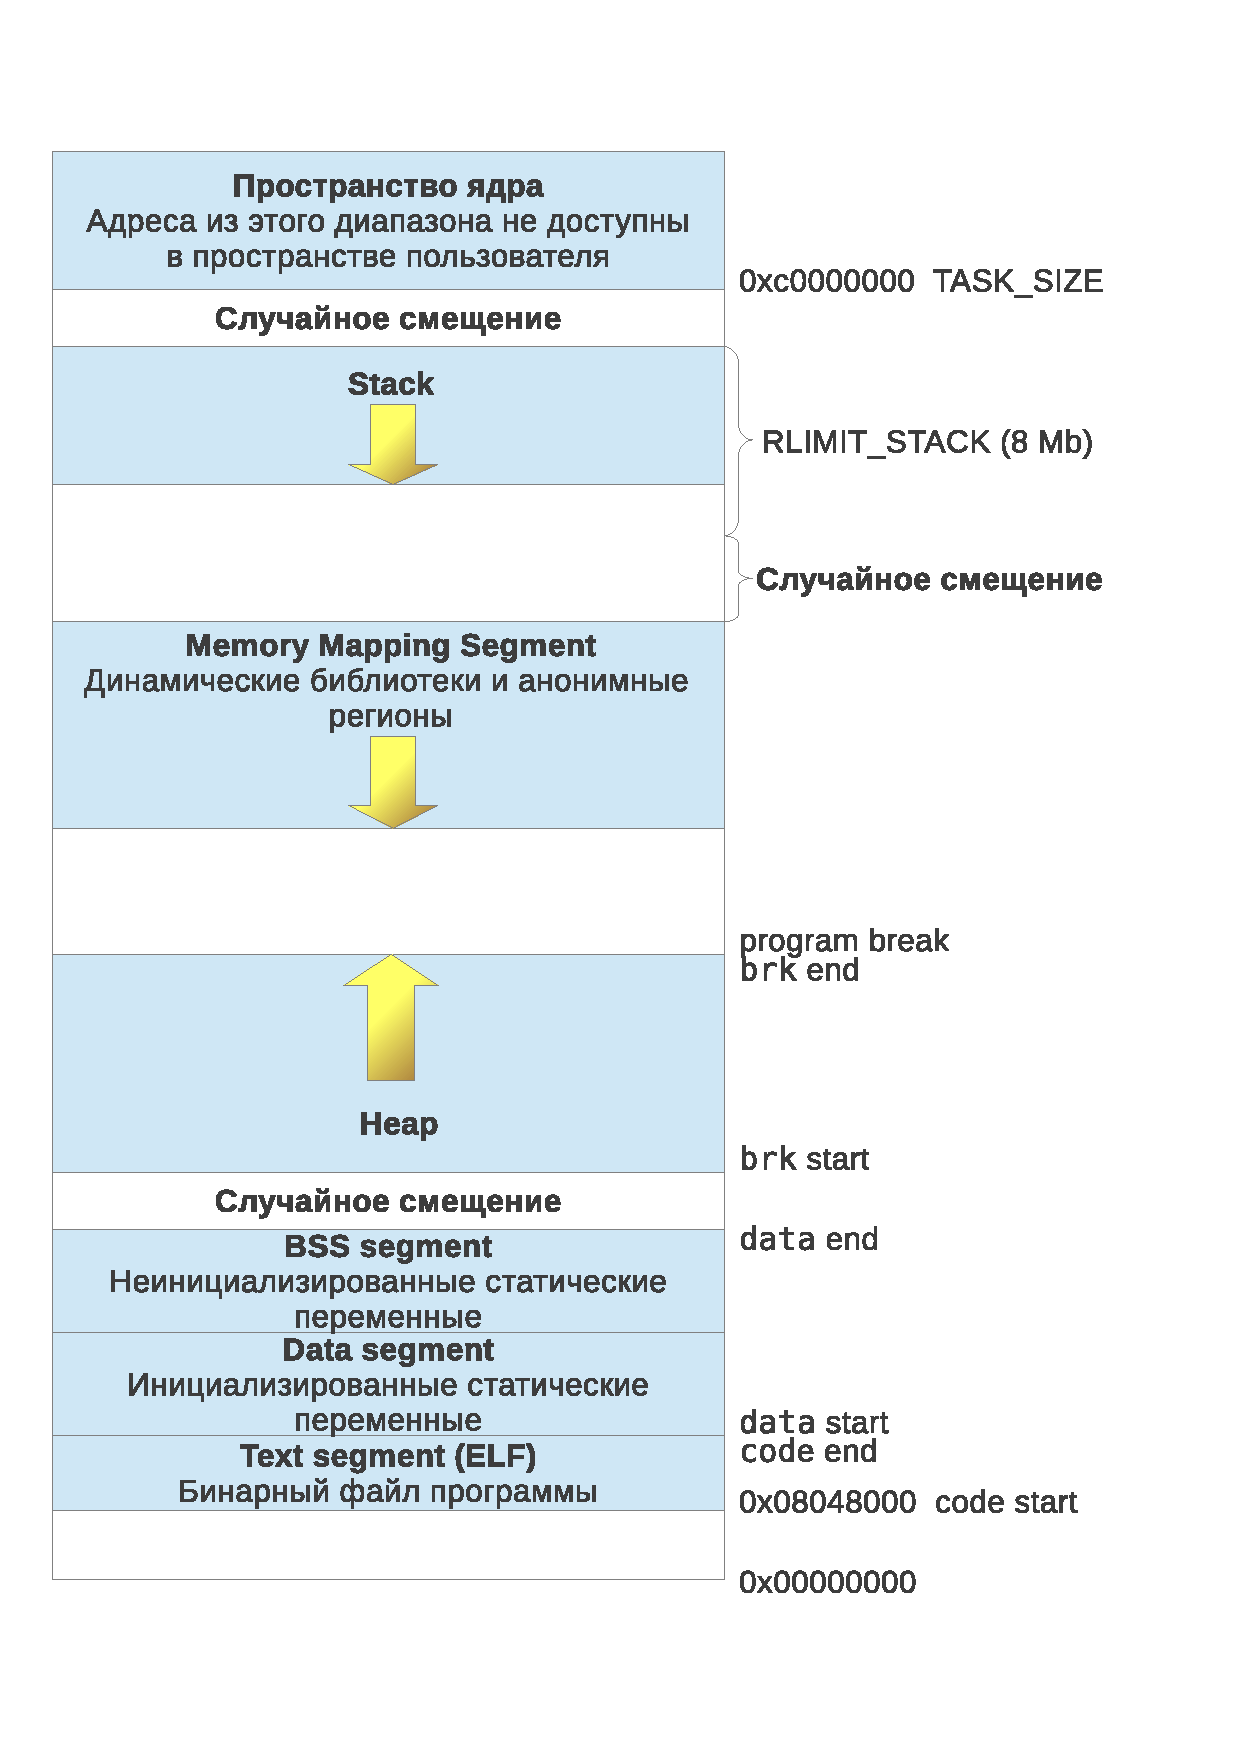
\includegraphics[width=0.6\linewidth]{memory_layout}}
\caption{Типичное размещение регионов памяти процесса ОС Linux на 32 разрядной архитектуре x86}
\label{pic:memory_layout}
\end{figure}

Основные поля описывающие структуру памяти процесса (см. листинг~\ref{code:mm_struct} и рис.~\ref{pic:memory_layout}):

\begin{itemize}

    \item mmap - указатель на голову списка дескрипторов регионов памяти процесса
    \item mmap\_base - указывает на начало Memory Mapping Segment.
    \item start\_code и end\_code описывают регион, в который был загружен код программы
    \item start\_data и end\_data описывают регион, в который были загружены данные
    \item start\_brk и brk описывают кучу процесса
    \item start\_stack указывает на начало сегмента стека программы

\end{itemize}

\subsection{Контекст процесса}

Контекст процесса описывает состояние процесса, в контекст входит следующая информация:

\begin{itemize}

    \item состояние регистров общего назначения
    \item состояние сопроцессоров и расширений (например, FPU, MMX/SSE)
    \item состояние сегментных регистров
    \item состояние управляющих регистров (например, cr3 или eflags)
    \item указатели стека и команд

\end{itemize}

В данной работе сохраняется минимальный набор информации, необходимый для восстановления процесса, который включает в себя регистры общего назначения (ebx, ecx, edx, esi, edi, ebp, eax), указатели стека и команд (esp и eip), а также регистр флагов (eflags).

\subsection{Файлы}

Файл, с точки зрения пользовательского приложения, просто неотрицательное число - файловый дескриптор и набор функций для манипулирования (open, close, read, write, ioctl и др.). Однако внутри операционной системы файлу может соответствовать как реальный файл хранящийся на диске так и виртуальный файл устройства, единый интерфейс является частью идеологии Unix - "все есть файл", однако состояния обычных файлов и файлов устройств описываются различными структурами и сохранятся должны по разному. Более того сохранение состояния файла устройства в общем виде вообще невозможно.

Стоит отметить, что файловый дескриптор может идентифицировать не только файлы, но и директории, сокеты, пайпы, общую память и различные другие ресурсы системы, состояние каждого из которых внутри ядра операционной системы описывается своей структурой, но пользователю для работы с ними предоставляются схожие интерфейсы.


\subsection{Сокеты}

Сокеты еще один важный ресурс процесса операционной системы Linux. Сохранение и восстановление состояния сокетов - это отдельная большая задача.

Сокеты, как правило, используются как интерфейс для организации сетевого взаимодействия, т. е. они затрагивают не только мигрируемый процесс, но и удаленный процесс, который ничего не знает о миграции. Кроме того, за интерфейсом сокетов скрывается сетевая подсистема Linux, которая поддерживает огромное количество разнообразных протоколов (каждый из которых может иметь свое состояние) и затрагивает большое количество других подсистем ядра.

Стоит также отметить, что интерфейс сокетов используется не только для организации сетевого взаимодействия, например, NETLINK сокеты используются для организации взаимодействия пользовательского процесса и ядра Linux (например, через NETLINK сокеты рассылается информация о подключенных к компьютеру usb устройствах).
